\chapter{MoonWire}
\label{chap:moonwire}

This Chapter describes the design and implementation of MoonWire, our VPN sandbox.
It is evaluated among the other VPNs in Chapter~\ref{chap:evaluation}.

\section{Design}
We wanted a modular, easy-to-change software that allows fast iteration and experimentation.
With MoonWire it is possible to rapidly try out different approaches to specific sub-problems.

\subsubsection{Protocol}
For the VPN protocol and data framing the WireGuard protocol is chosen due to its minimal design. Only 3 types of message frames are needed to create a new channel and exchange data.

MoonWire aims the be compatible with WireGuard, but does not reach this goal in some aspects. The cookie response mechanism for DoS protection and re-keying timers are not implemented.
WireGuard's replay window of 2000 slots is sometimes to small to capture the reordering effects of having independent worker threads.

\subsubsection{Software}
%DPDK as basis, libmoon, libsodium, blake2s reference impl
Previous research and our own measurements in Section~\ref{EVAL} showed that the network and driver stack of the OS can be a limiting factor due to its generality and some architectural limitations~\cite{TODO}.
To work around this bottleneck and to gain a high configurability, MoonWire is based on the user-space packet processing framework DPDK. It comes with high-performance NIC drivers and an abundance of specialized data structures for packet processing tasks. Since DPDK applications are written in C/C++, they require a certain amount of boilerplate code, which can ge greatly reduce by using libmoon, a high-level Lua wrapper around DPDK.

For cryptographic primitives the open-source libsodium library~\cite{libsodium-website}  is used. It is a cross-platform collection of high-security, but none the less fast implementations, provided behind an easy-to-use, hard-to-get-wrong API.
and has several benefits over rolling your own implementations.

The exact versions of all used software is given in Table~\ref{TODO}.

\section{Implementation}
%Present tried common implementation approaches that are possible, explain trade-offs, benchmark different versions, justify the final choice
Since the evaluated state-of-the art VPN solutions made vastly different design choices, it made sense to not concentrate on a single implementation. In the following variants we replicate seen designs and present a new one. Each one is explained from the high-level design to the specific implementation details.

\subsection{Details / Data Structures}

\subsubsection{Peer Table}

To check if an incoming packet is to be processed, some form of lookup data structure is needed. Depending on the specification of the protocol, different options are possible. 
WireGuard identifies interesting packets on the destination IP address, by checking them against the configured subnets of allowed IPs. IPsec is more complex in this regard and also allows filters on ports and source addresses.
IP address lookup tables are an extensively studied field~\cite{} with many established high-performance implementations.
For MoonWire we rely in the LPM library of DPDK, which uses the DIR-24-8 algorithm for its IPv4 table.

\subsubsection{Peer State}

The peer state encapsulates all information necessary to send and receive packets from a remote VPN peer. It must contain the cryptographic key material, the address of the remote endpoint and the nonce counter.
Functionally it is comparable to security associations (SAs) in IPsec.

\begin{lstlisting}[caption={Definition of the peer struct without locks},captionpos=b,label={lst:moonwire-peer-struct},language=C]
struct peer_no_lock {
	uint8_t rxKey[crypto_aead_chacha20poly1305_IETF_KEYBYTES];
	uint8_t txKey[crypto_aead_chacha20poly1305_IETF_KEYBYTES];
	uint8_t nonce[crypto_aead_chacha20poly1305_IETF_NPUBBYTES];
	uint32_t id;
	union ip4_address endpoint;
	uint16_t endpoint_port;
	/* rte_spinlock_t lock_; */
};
\end{lstlisting}

While the values like the endpoint or keys are set once and then mostly read, the nonce counter is updated for every packet. For this to be thread-safe with multiple parallel workers, a lock can be added to the structure in Listing~\ref{lst:moonwire-peer-struct}. Compared to a global or table-wide lock, this allows concurrent operation of workers, as long as they access different peer states.

%\subsubsection{Packet Distribution}
%Packets arrive at a RxQueue of a device and have to be dequeued and processed.
%Multiple options, pipelines, queues and stuff
%
%Note: For the gateway usecase (1:1) RSS does not work since src and dst ip/port are equal on every packet. It can work in multi-client setup.


%\subsubsection{Replay Protection}


\subsubsection{A Note on Nonce Handling}
Nonce counters used as IVs play an important role in protecting the confidentiality in symmetric ciphers. 
In the case of AES-GCM forgery attacks become possible if a nonce is reused under a given key~\cite{dworkin2007recommendation}. The same applies to the IETF version of the ChaCha20 cipher~\cite{TODO}.
NIST mandates, that the probability of this occurring must be smaller than $2^{-32}$ in conforming implementations~\cite{dworkin2007recommendation}.

For uniformly, randomly generated nonces, this probability is a generalized form of the birthday problem and can be calculated by Equation~\ref{eq:birthday-prob}, where the nonces are the days and the packets replace people.

\begin{equation}
p(\textrm{packets}, \textrm{bits}) = 1 - \frac{\textrm{packets}! \times \binom{2^\textrm{bits}}{\textrm{packets}}}{
	{(2^\textrm{bits})}^\textrm{packets}
}
\label{eq:birthday-prob}
\end{equation}

Calculating binomial coefficients of large numbers is computationally expensive. Therefore, the above formula can be approximated by the Taylor series expansion of the exponential function~\cite{TODO}:

\begin{equation}
p(\textrm{packets}, \textrm{bits}) = 1 - e^{- \frac{\textrm{packets}(\textrm{packets}-1)}
	{2^\textrm{bits}*2}}
\label{eq:birthday-prob-approx}
\end{equation}

Figures~\ref{fig:collisionprob1mpps} (a) and (b) plot Equation~\ref{eq:birthday-prob-approx} for a constant packet rate of 1 Mpps and nonces of 128 and 96 bit size. The horizontal line shows the NIST recommended maximum risk of $2^{-32}$. On the x-axes the number of transmitted packets in hours are given. Note that both axes are logarithmic. 

\begin{figure}[h]
	\centering
	\subfloat[192 bit nonce, XChacha20]{%
		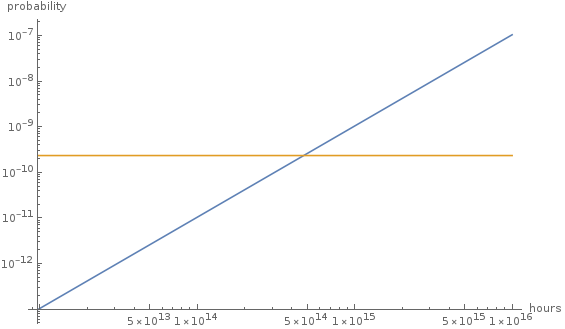
\includegraphics[height=0.25\linewidth]{figures/collision_prob_1mpps_192_bits}
		\label{fig:collisionprob1mpps192bits}
	}
	\subfloat[96 bit nonce, AES-GCM \& ChaCha20]{%
		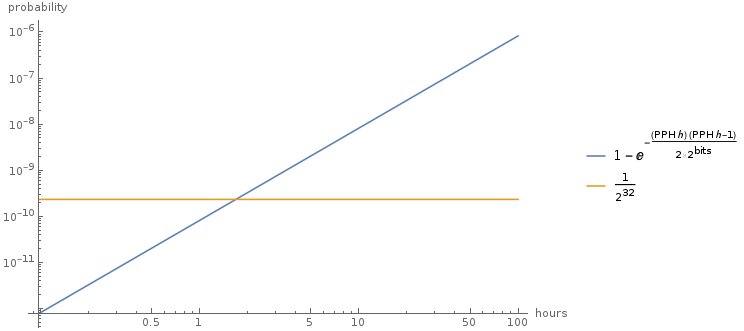
\includegraphics[height=0.25\linewidth]{figures/collision_prob_1mpps_96_bits}
		\label{fig:collisionprob1mpps96bits}
	}
	\caption{Collision probabilities of randomly generated nonces at 1 Mpps}
	\label{fig:collisionprob1mpps}
\end{figure}

%WireGuard protocol specifies IETF chacha20poly1507 with 12 (recheck this) bytes nonces. Since nonce reuse under the same key is devastating for security, implementations have to ensure this never happens. For short nonces it is recommended to increment the previous one, instead of generating random ones.

For 96 bit nonces, like used in AES-GCM (IPsec) and IETF-ChaCha20 (WireGuard), the threshold is passed in under 2 hours of traffic.
This concludes why random generation of small nonces is not recommended. Instead, it is usual to keep the last number and increment it with each packet. In multi-threaded implementations this can become a bottleneck as the nonces are essentially shared state between multiple read-write threads and have to be synchronized.

An possible solution to this problem could be the usage of ciphers with larger nonces, such as XChaCha20. The enlarged value range decreases the probability of collisions over-proportionally, as seen in Figure (b). There it takes $4\times 10^{14}$ hours to reach the same risk level as above. An equivalent of 10 times the age of the sun.

%The following describes different techniques to solve this.
%Note: As an alternative using XChacha20, 192-bit nonce, can be randomly generated, no shared state

%\subsubsection{Mutual exlusive access (atomics, mutex, \texttt{\_\_sync\_add\_and\_fetch()})}
%\subsubsection{One Thread maintains nonces, sends them with work packet}
%\subsubsection{Partitioning}

%\subsubsection{AVX512}
%Intel CPUs throttle frequency if AVX512 (?) code is encountered, this P-state change takes time + the rest of the code runs at slower base frequency.
%Implement this, check freqs, benchmark, see if AVX512 can be worth it.

%


\subsection{Variant 1 - Naive Single Instance}
The first variant is based on the design of OpenVPN and conceptually simple. The whole application consists of a single thread, that completes all tasks of VPN operation.

\begin{figure}[h]
	\centering
	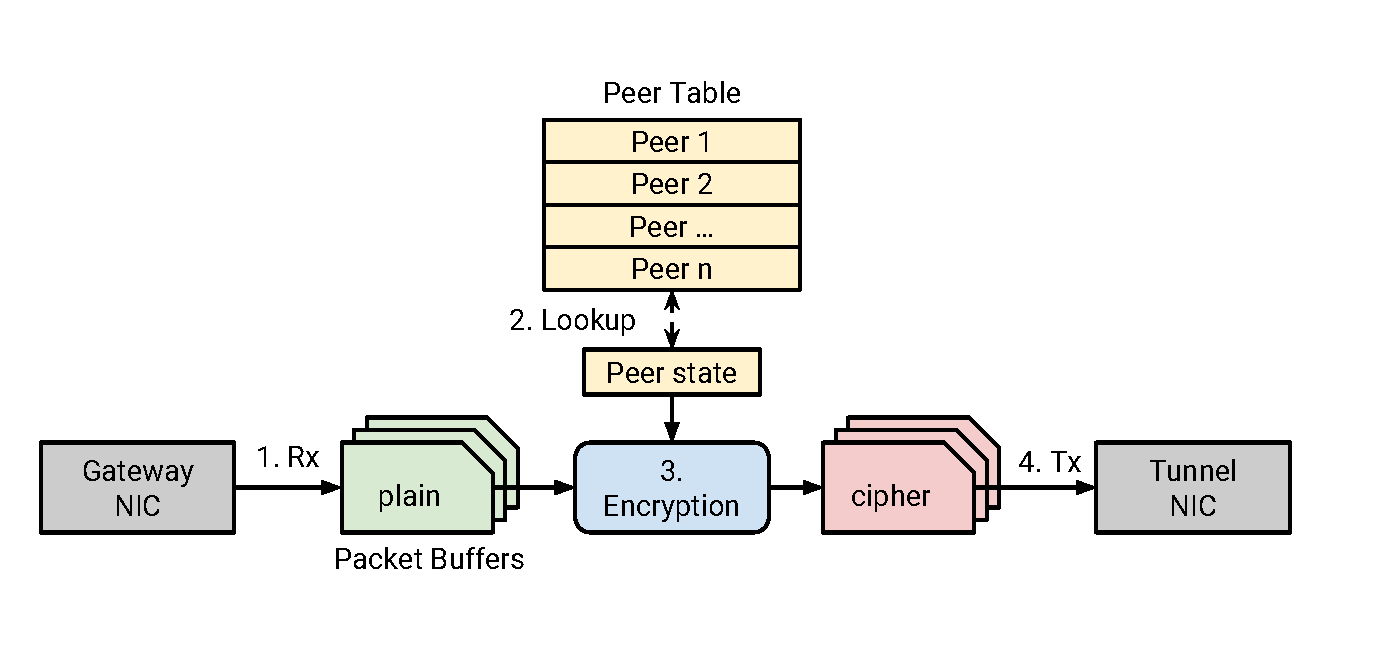
\includegraphics[width=0.9\linewidth]{figures/moonwire-variant-1}
	\caption{Flowchart of MoonWire variant 1}
	\label{fig:moonwire-variant-1}
\end{figure}

In Figure~\ref{fig:moonwire-variant-1} the different steps in the continuous main loop of variant 1 are visualized. The thread starts by receiving incoming packet from the gateway interface in form of a batch of \texttt{rte\_pktbufs}. Each buffer is validated and the associated peer state is looked up in the peer table. If there is a running connection, the buffer is extended, encrypted and new IP headers are inserted. In the last step, all valid packets are send and the remaining ones are freed, thus reclaiming their descriptors and memory into the pool of the gateway.

Due to its single-threaded nature, there is no need for any kind of synchronization on the peer table or state. This simplifies the state-keeping process greatly and poses the least requirements on the used data structures. A simple LPM table such as the one provided by DPDK~\cite{dpdk-lpm-api} can be used to implement the peer table.
This variant does also no suffer from averse traffic pattern, like single-flow traffic. With only one thread, there are no benefits in using RSS and multiple queues. Therefore, uneven packet distribution can not occur. On the contrary, such traffic could even be beneficial, since repeated lookups of the same value utilizes the CPU caches better than different addresses, which generate repeated cache misses and evictions.

On the downside, this variant shares its drawbacks with OpenVPN. Namely, the total lack of horizontal scaling. Other cores can only be utilized by spawning multiple independent instances and fragmenting the routed subnets into smaller chunks.


\subsection{Variant 2 - Independent Workers}
Variant 2 takes the crude scaling attempts necessary for variant 1 or OpenVPN and internalizes them. In summary, this version is most similar to IPsec in the Linux Kernel.

\begin{figure}[h]
	\centering
	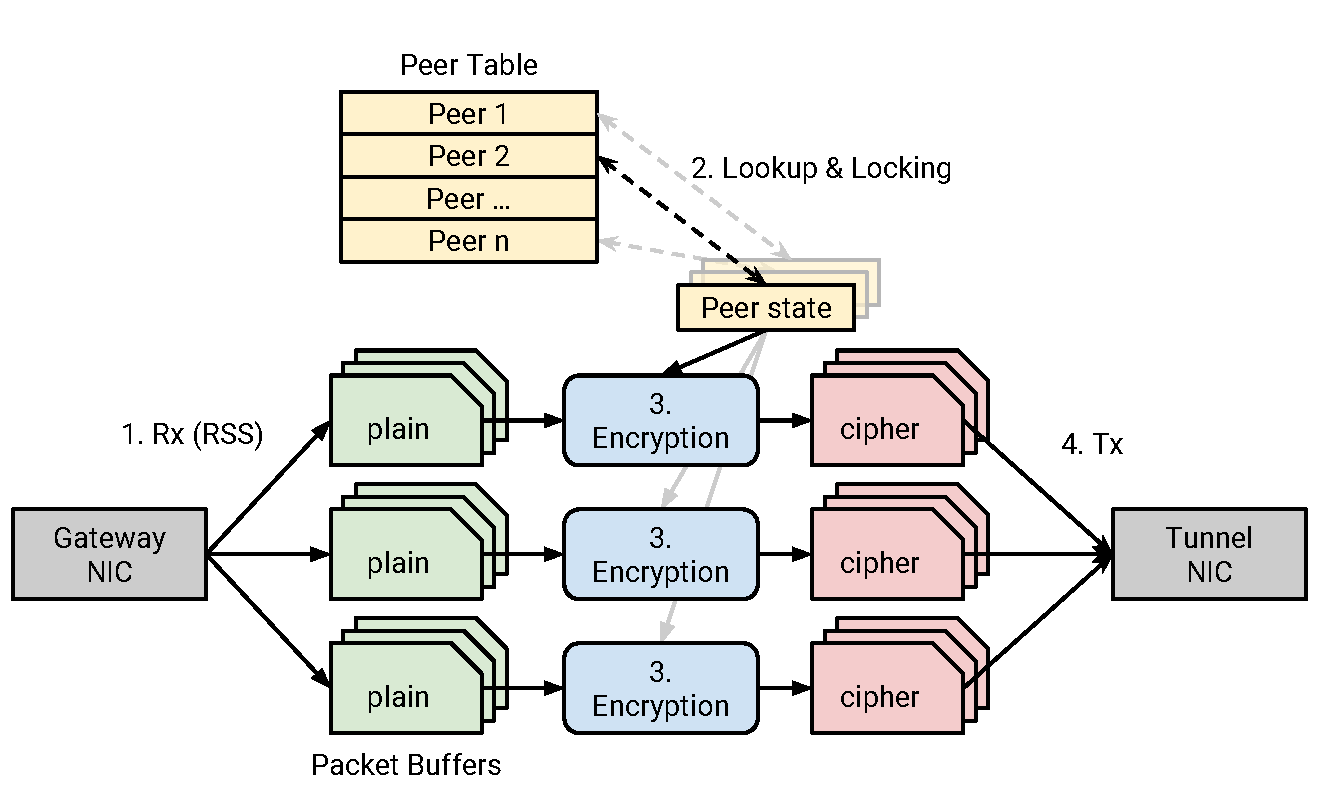
\includegraphics[width=0.9\linewidth]{figures/moonwire-variant-2}
	\caption{Flowchart of MoonWire variant 2}
	\label{fig:moonwire-variant-2}
\end{figure}

As seen in Figure~\ref{fig:moonwire-variant-2}, multiple workers are processing the packets in parallel, each with its own NIC queues. Each worker still completes the whole loop from reception, encryption to transmission. Incoming packets are distributed to multiple queues on the hardware level by the NIC through RSS.
Since there are multiple threads accessing and modifying shared data, data accesses have to be synchronized to prevent corruption. 
The DPDK LPM lookup table is not thread-safe for performance reasons, but read-only lookups can be performed from multiple threads at the same time~\cite{dpdk-fastpath-api}. Fortunately, changes to the table structure are rare, namely when the VPN configuration is modified, so this operation is allowed to be more expensive and slow. 
The peer state, on the other hand, is written to for every packet when the nonce is incremented. In our implementation it is secured by a traditional lock, which a worker thread takes before encrypting an entire batch of packets and releases it afterwards.

There exist many implementations of locks. We take the classic \texttt{pthread\_mutex} from the POSIX threading library and compare it to the \texttt{rte\_spinlock} provided by DPDK, henceforth called variant 2a and 2b respectively. The POSIX mutex internally relies on \texttt{futex} API of the Kernel and is a general purpose lock. In particular, when waiting for a lock to be become free, the calling threads is suspended and does not consume further cycles.
Spinlocks, on the other hand, do not relinquish control to the scheduler, but continuously keep trying. 
This trades latency for energy efficiency, and to some degree performance under heavy contention, as seen in the evaluation~\ref{TODO}.  


\subsection{Variant 3 - Work Pipeline}
In variant 3 the best properties of the previous versions are taken, while avoiding their drawbacks. 
Variant 1 showed, that not utilizing multiple cores will limit performance greatly, as operations like encryption of large buffers inherently need much processing power.
A shared peer state with locks, as implemented in variant 2, inhibits scaling too much, by introducing synchronization overhead, to be viable. 

\begin{figure}[h]
	\centering
	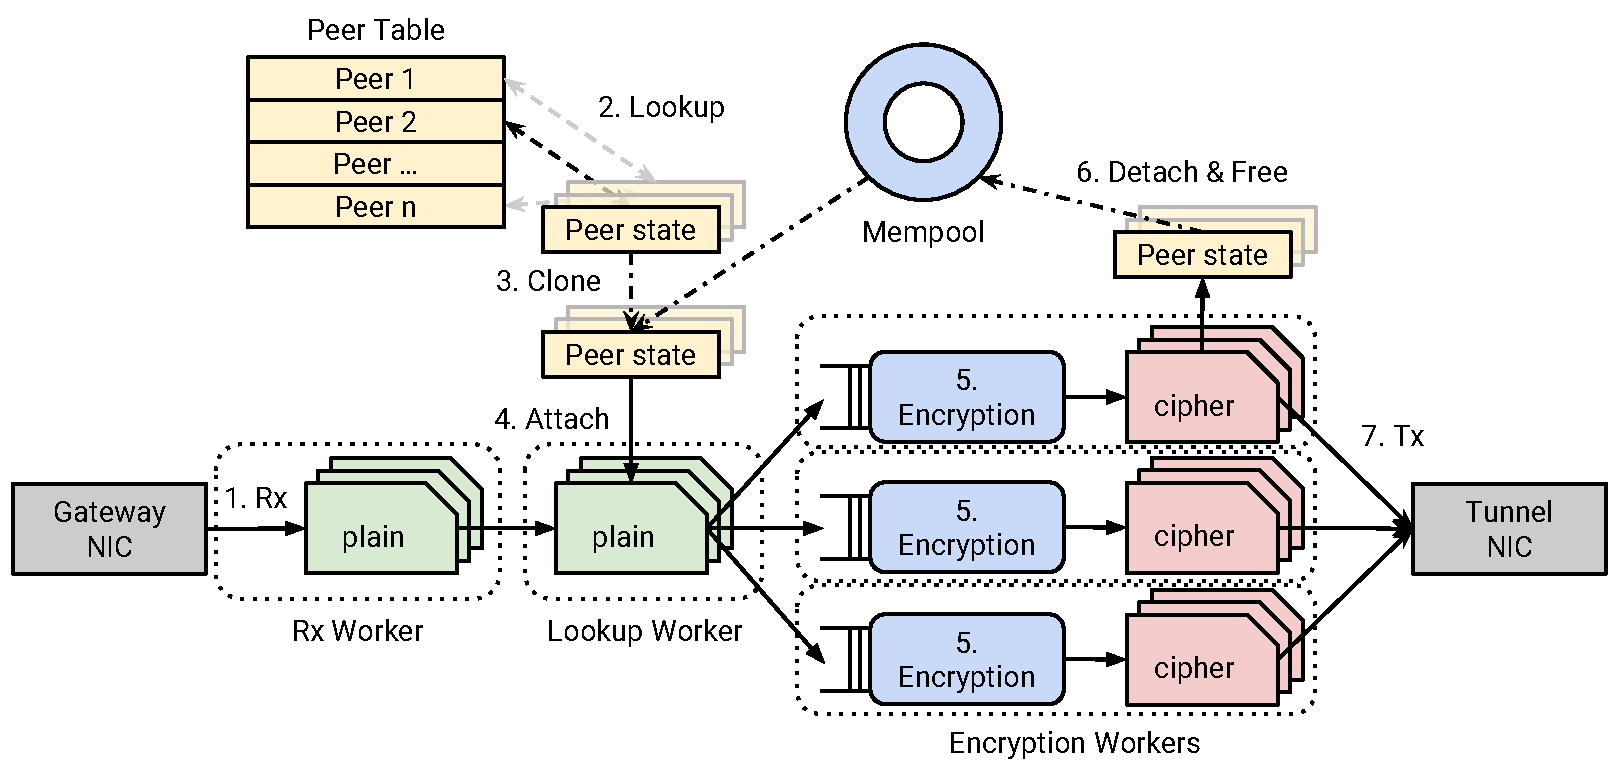
\includegraphics[width=1\linewidth]{figures/moonwire-variant-3}
	\caption{Flowchart of MoonWire variant 3}
	\label{fig:moonwire-variant-3}
\end{figure}

Therefore, a hybrid approach in chosen for variant 3. The peer table and state is still contained in and maintained by a single thread, therefore lock-free, while the encryption stage is parallelized across multiple workers. Instead of handing out mutable peer state references to the workers, the state is cloned and distributed in a message passing manner.
A lookup worker fetches the applicable state to a packet buffer, increments the nonce counter, copies the entire state with all keys and endpoint information into a separate empty buffer, and attaches this buffer to the packet buffer. The \texttt{rte\_membuf} struct includes a member field called \texttt{udata64} for this purpose. The parallel workers now find all information needed for encryption contained in the packet buffer and do not have to updated any shared state.
Since this crypto-args buffer is separate allocated memory, it has to be reclaimed after use. Traditional memory management with \texttt{malloc()/free()} is to slow to be used a million times per second concurrently~\cite{TODO}. Therefore it is implemented the same way as the packet buffers; as fixed-sized, memory-pooled data buffers. 
DPDK exposes the packet buffer memory pools as plain \texttt{rte\_mempools} without the network packet specific customization, so we use them here.

Buffer distribution between the stages happen through DPDK \texttt{rte\_rings}; lock-free, FIFO, high performance queues with batched functions to reduce overhead. 
The step from the lookup to the encryption workers could be solved by having one MPMC queue, but this introduces more shared state than multiple SPSC queues. For one, SPSC semantics allow DPDK to use more relaxed and faster enqueue/dequeue functions without an atomic CMP-XCHG loop~\cite{dpdk-rte-ring-enqueue}. It also reduces false sharing cache evictions caused by dequeues from other workers. Overall this trades memory usage for performance. Distribution over the workers happens in a round-robin fashion to ensure equal load among them.


In a previous version the Rx and the Lookup worker where unified into one. But as shown in Figure~\ref{}, there is a significant amount of time spend for state cloning. To speed this process up, packet reception has been factored out in the final design shown in Figure~\ref{fig:moonwire-variant-3}.
